\documentclass{scrreprt}

\usepackage[german]{babel}
\usepackage{fourier}
\usepackage[utf8]{inputenc}
\usepackage[T1]{fontenc}
\usepackage{amsfonts,amsthm, amsmath}
\usepackage{listings}
% The following is needed in order to make the code compatible
% with both latex/dvips and pdflatex.
\ifx\pdftexversion\undefined
\usepackage[dvips]{graphicx}
\else
\usepackage[pdftex]{graphicx}
\DeclareGraphicsRule{*}{mps}{*}{}
\fi

\setlength\parindent{0pt}
\lstset{language=Erlang}

\begin{document}

\textbf{Team:} Falco Winkler (FW), Daniel Schruhl (DS)\\
\\
\textbf{Aufgabenteilung:}\\

\textbf{Quellenangaben:}\\
\\
\textbf{Bearbeitungszeitraum:}
\begin{itemize}
	\item 26.03.2017 (FW,DS)
\end{itemize}

\textbf{Aktueller Stand:}\\

\textbf{Änderung des Entwurfs:}\\

\textbf{Entwurf:}\\
Sequenzdiagramm
\begin{figure}[!htb]
\centering
	\includegraphics[width=\textwidth]{sequence-diagram.png}
\caption[seq-dia]{Sequenzdiagramm bei fehlerfreiem Nachrichtenaustausch}
\label{fig:sequence-diagram}
\end{figure}

Komponentendiagramm
\begin{figure}[!htb]
\centering
	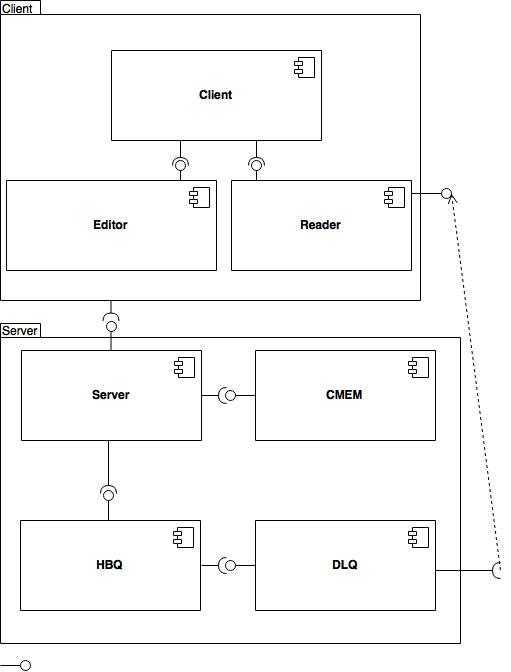
\includegraphics[width=\textwidth]{component-diagram.png}
\caption[seq-dia]{Komponentendiagramm der Message Of The Day App}
\label{fig:component-diagram}
\end{figure}

\end{document}